\clearpage
\section{Design Choices}
\subsection{Detection interface}
\begin{figure}[H]
    \centering
    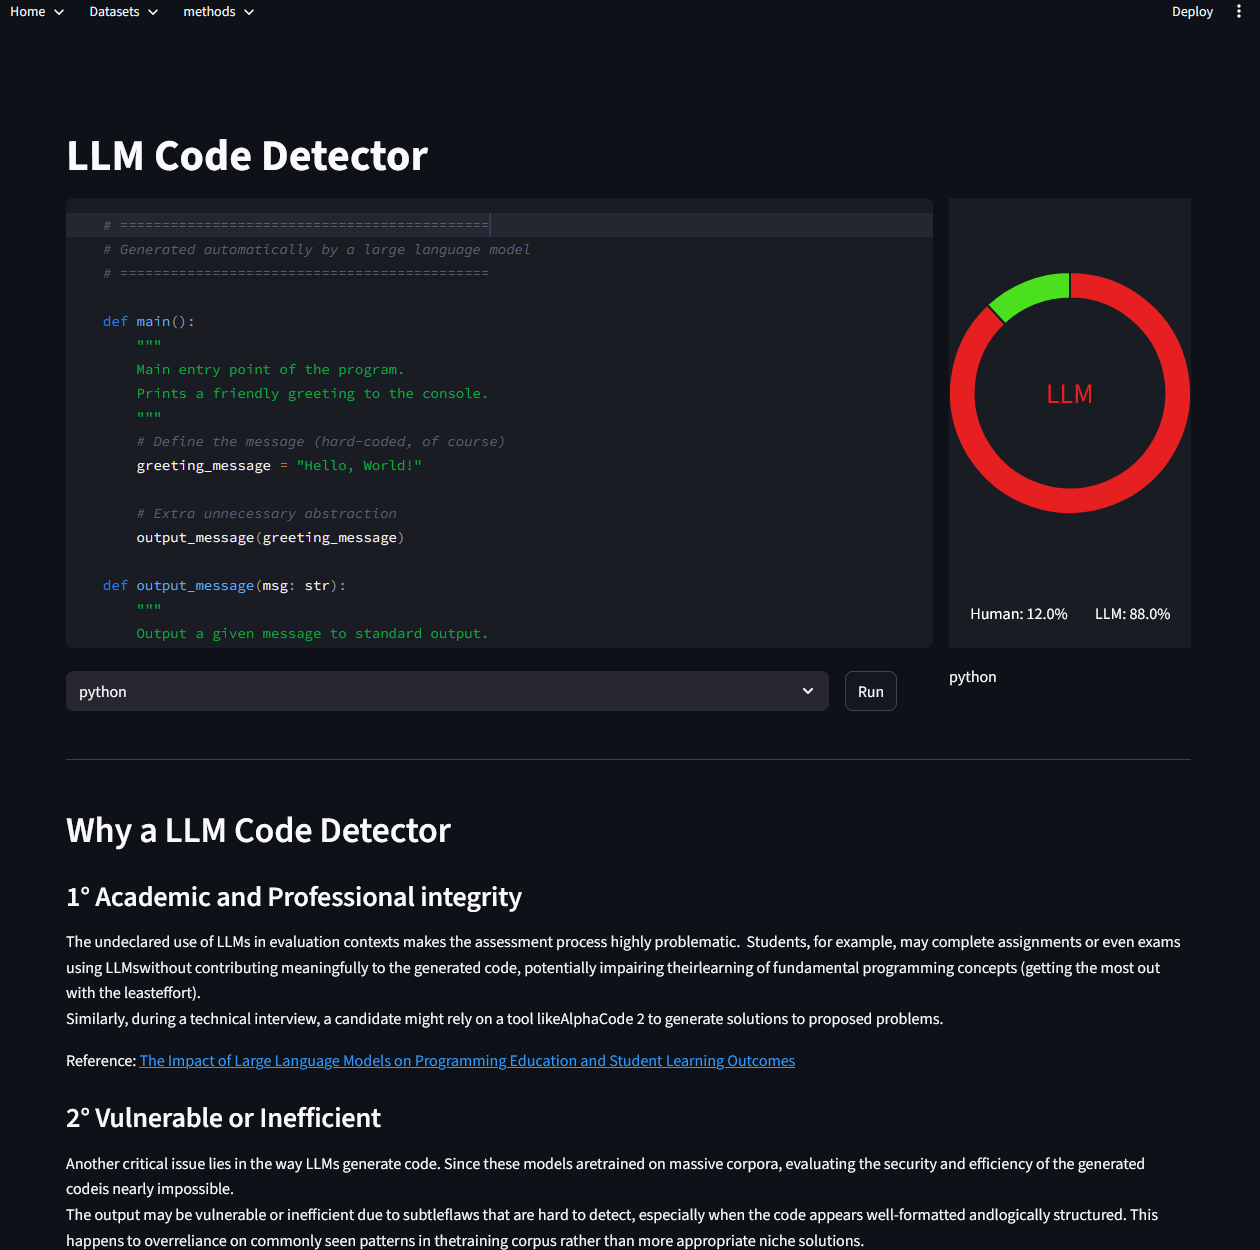
\includegraphics[width=0.8\linewidth]{img/interfaccia/Screenshot 2025-09-27 172409.png}
    \caption{detection interface}
    \label{fig:gptzeroe}
\end{figure}
It was decided to design the text box to recognize programming 
language patterns and allow the code to be displayed in a 
user-friendly manner according to the programming language. 
For this reason, a section was added to select the 
language of the code. 
Language selection also allows the \textit{“code cleaner”} to more easily recognize 
comments and indentation to remove. It also enables syntax highlighting 
according to the selected language. 

After entering the code on the right, after a brief loading period, 
the probability that the code was generated by an LLM or written by 
a human will be displayed. The percentage bar changes colour 
depending on the percentage. On the same page, the reasons why an LLM code detector 
is useful are quickly listed.

Additionally, at the bottom of the page it is possible to read the 
reasons why an LLM code detector is useful and necessary (the same 
reasons presented in this thesis).

\subsection{Dataset interface}
\begin{figure}[H]
    \centering
    \begin{subfigure}[t]{0.45\textwidth}
        \centering
        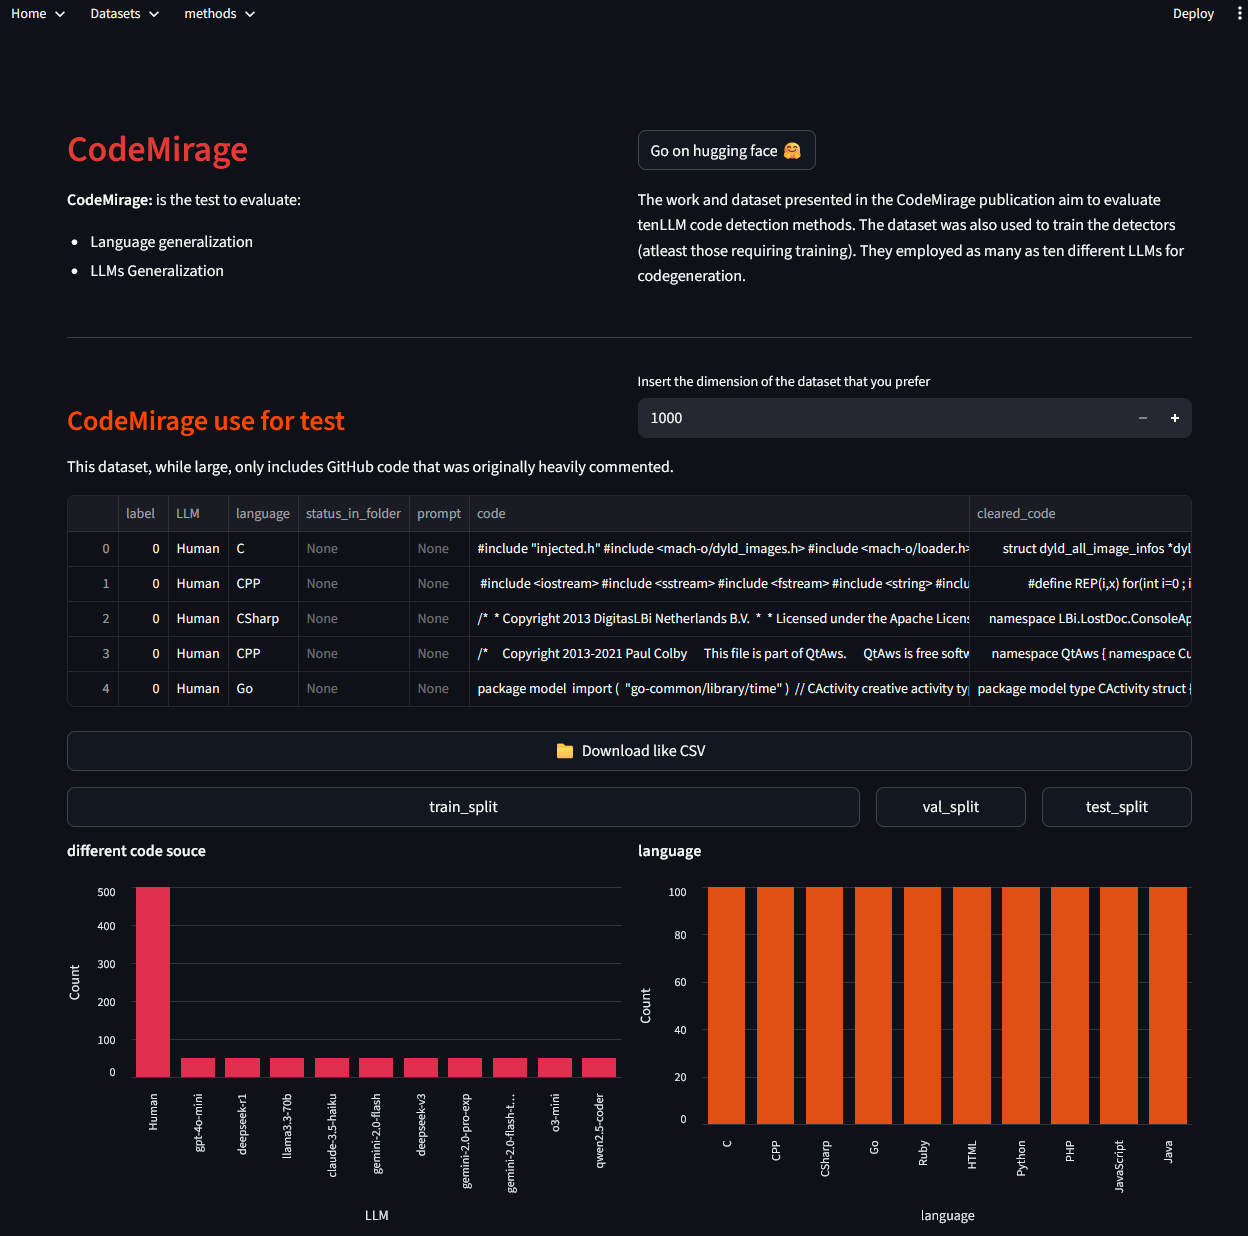
\includegraphics[width=\linewidth]{img/interfaccia/Screenshot 2025-09-27 172512.png}
        \caption{CodeMirage dataset interface}
        \label{fig:errit}
    \end{subfigure}
    \hfill
    \begin{subfigure}[t]{0.45\textwidth}
        \centering
        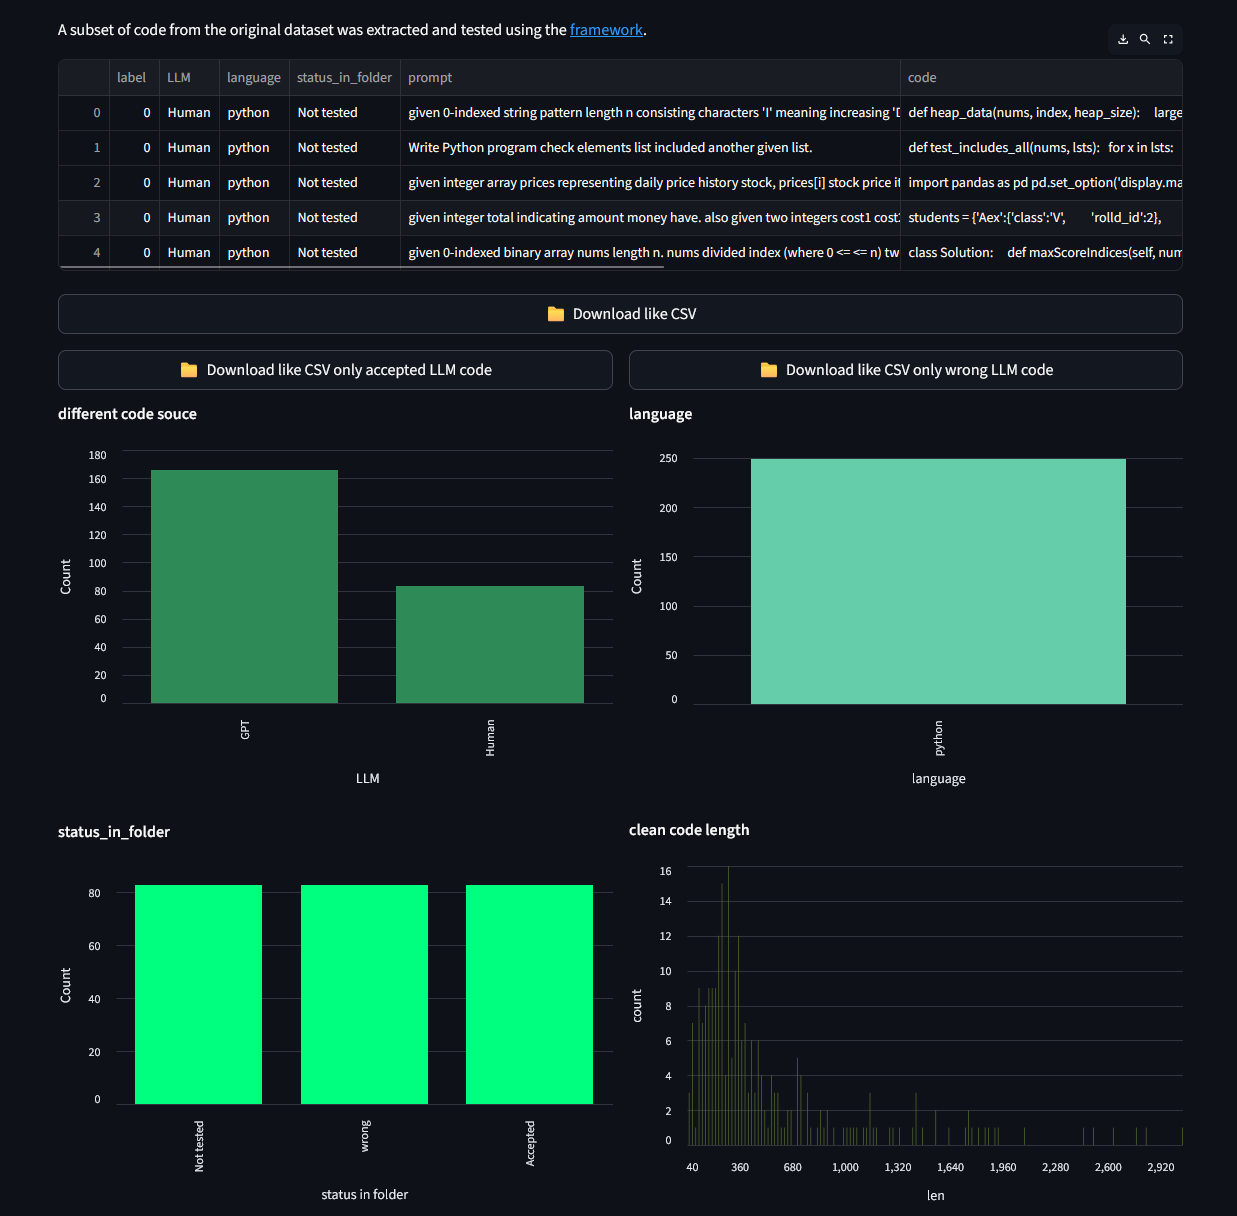
\includegraphics[width=\linewidth]{img/interfaccia/Screenshot 2025-09-27 172541.png}
        \caption{Pan dataset interface}
        \label{fig:ab2sceyg}
    \end{subfigure}
\end{figure}

%%%%%%%%%%%%%%%%%
In the dataset section, every dataset available from Hugging 
Face is automatically downloaded. The purposes for which the 
dataset is recommended for use are provided (for example, AIG 
is recommended for testing the detection method's ability to 
identify competitive code).

Users are also given the option to decide the size of the 
subset they wish to obtain from the dataset. A balanced subset 
is then automatically created based on: LLM generators, 
programming languages, and code correctness. When these 
fields are not present, they are ignored. Additionally, a 
graph is displayed to visually represent the average length 
of code without comments.

\clearpage
\subsection{Testing Methods interface}
\begin{figure}[H]
        \centering
        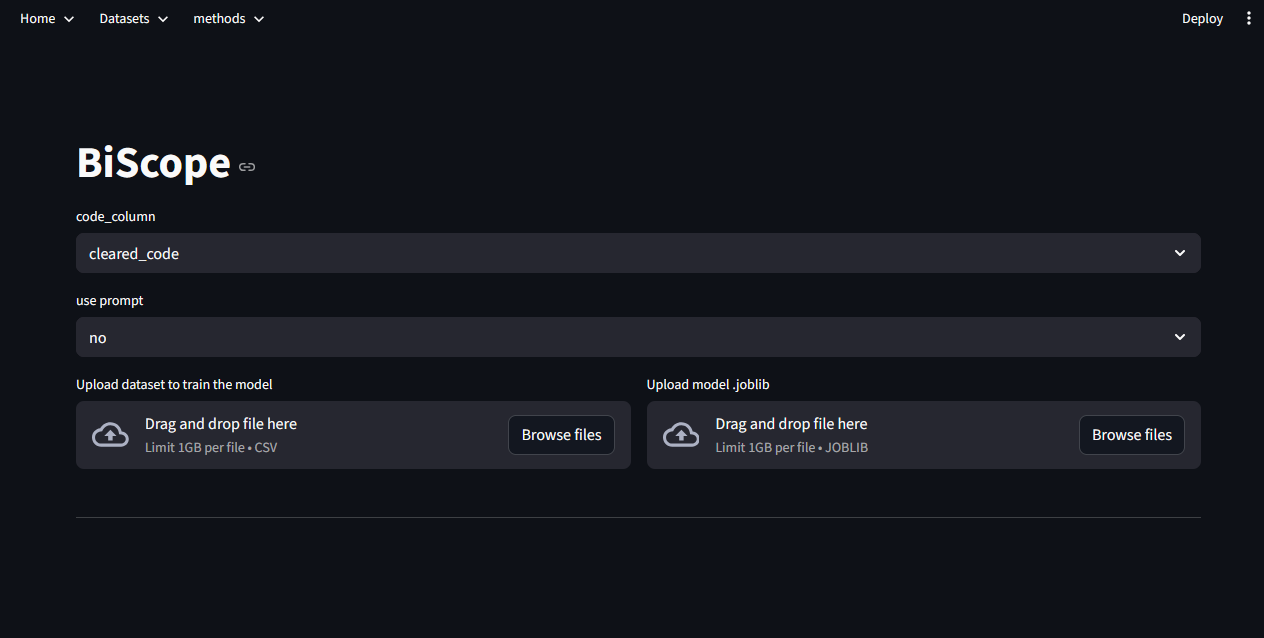
\includegraphics[width=0.8\linewidth]{img/interfaccia/Screenshot 2025-09-27 172640.png}
        \caption{Biscope interface}
        \label{fig:errit}
\end{figure}

The interface for each method is different because each method requires 
different information. For example, perplexity-based methods have an interface 
to set and compute the best probability threshold and to run tests. 
Machine-learning-based models have an interface to train or load a 
pre-trained model and then test it on a new dataset. Obviously, 
the user cannot load any test dataset without first loading a model 
or the threshold.
The possible test settings can be quickly recalled:
\begin{enumerate}
\item Select whether to test/train on raw code or clean code.
\item BiScope allows the use of problem descriptions for creating the test on which perplexity is evaluated (option not used during the reported tests).
\item CodeT5 allows the use of quantization at inference and LoRA during training.
\item LLMPPL allows setting a preferred threshold or calculating the best threshold on a “training” dataset.
\end{enumerate}
%%%%%%%%%%%%%%%%%